\documentclass[1p]{elsarticle_modified}
%\bibliographystyle{elsarticle-num}

%\usepackage[colorlinks]{hyperref}
%\usepackage{abbrmath_seonhwa} %\Abb, \Ascr, \Acal ,\Abf, \Afrak
\usepackage{amsfonts}
\usepackage{amssymb}
\usepackage{amsmath}
\usepackage{amsthm}
\usepackage{scalefnt}
\usepackage{amsbsy}
\usepackage{kotex}
\usepackage{caption}
\usepackage{subfig}
\usepackage{color}
\usepackage{graphicx}
\usepackage{xcolor} %% white, black, red, green, blue, cyan, magenta, yellow
\usepackage{float}
\usepackage{setspace}
\usepackage{hyperref}

\usepackage{tikz}
\usetikzlibrary{arrows}

\usepackage{multirow}
\usepackage{array} % fixed length table
\usepackage{hhline}

%%%%%%%%%%%%%%%%%%%%%
\makeatletter
\renewcommand*\env@matrix[1][\arraystretch]{%
	\edef\arraystretch{#1}%
	\hskip -\arraycolsep
	\let\@ifnextchar\new@ifnextchar
	\array{*\c@MaxMatrixCols c}}
\makeatother %https://tex.stackexchange.com/questions/14071/how-can-i-increase-the-line-spacing-in-a-matrix
%%%%%%%%%%%%%%%

\usepackage[normalem]{ulem}

\newcommand{\msout}[1]{\ifmmode\text{\sout{\ensuremath{#1}}}\else\sout{#1}\fi}
%SOURCE: \msout is \stkout macro in https://tex.stackexchange.com/questions/20609/strikeout-in-math-mode

\newcommand{\cancel}[1]{
	\ifmmode
	{\color{red}\msout{#1}}
	\else
	{\color{red}\sout{#1}}
	\fi
}

\newcommand{\add}[1]{
	{\color{blue}\uwave{#1}}
}

\newcommand{\replace}[2]{
	\ifmmode
	{\color{red}\msout{#1}}{\color{blue}\uwave{#2}}
	\else
	{\color{red}\sout{#1}}{\color{blue}\uwave{#2}}
	\fi
}

\newcommand{\Sol}{\mathcal{S}} %segment
\newcommand{\D}{D} %diagram
\newcommand{\A}{\mathcal{A}} %arc


%%%%%%%%%%%%%%%%%%%%%%%%%%%%%5 test

\def\sl{\operatorname{\textup{SL}}(2,\Cbb)}
\def\psl{\operatorname{\textup{PSL}}(2,\Cbb)}
\def\quan{\mkern 1mu \triangleright \mkern 1mu}

\theoremstyle{definition}
\newtheorem{thm}{Theorem}[section]
\newtheorem{prop}[thm]{Proposition}
\newtheorem{lem}[thm]{Lemma}
\newtheorem{ques}[thm]{Question}
\newtheorem{cor}[thm]{Corollary}
\newtheorem{defn}[thm]{Definition}
\newtheorem{exam}[thm]{Example}
\newtheorem{rmk}[thm]{Remark}
\newtheorem{alg}[thm]{Algorithm}

\newcommand{\I}{\sqrt{-1}}
\begin{document}

%\begin{frontmatter}
%
%\title{Boundary parabolic representations of knots up to 8 crossings}
%
%%% Group authors per affiliation:
%\author{Yunhi Cho} 
%\address{Department of Mathematics, University of Seoul, Seoul, Korea}
%\ead{yhcho@uos.ac.kr}
%
%
%\author{Seonhwa Kim} %\fnref{s_kim}}
%\address{Center for Geometry and Physics, Institute for Basic Science, Pohang, 37673, Korea}
%\ead{ryeona17@ibs.re.kr}
%
%\author{Hyuk Kim}
%\address{Department of Mathematical Sciences, Seoul National University, Seoul 08826, Korea}
%\ead{hyukkim@snu.ac.kr}
%
%\author{Seokbeom Yoon}
%\address{Department of Mathematical Sciences, Seoul National University, Seoul, 08826,  Korea}
%\ead{sbyoon15@snu.ac.kr}
%
%\begin{abstract}
%We find all boundary parabolic representation of knots up to 8 crossings.
%
%\end{abstract}
%\begin{keyword}
%    \MSC[2010] 57M25 
%\end{keyword}
%
%\end{frontmatter}

%\linenumbers
%\tableofcontents
%
\newcommand\colored[1]{\textcolor{white}{\rule[-0.35ex]{0.8em}{1.4ex}}\kern-0.8em\color{red} #1}%
%\newcommand\colored[1]{\textcolor{white}{ #1}\kern-2.17ex	\textcolor{white}{ #1}\kern-1.81ex	\textcolor{white}{ #1}\kern-2.15ex\color{red}#1	}

{\Large $\underline{12n_{0002}~(K12n_{0002})}$}

\setlength{\tabcolsep}{10pt}
\renewcommand{\arraystretch}{1.6}
\vspace{1cm}\begin{tabular}{m{100pt}>{\centering\arraybackslash}m{274pt}}
\multirow{5}{120pt}{
	\centering
	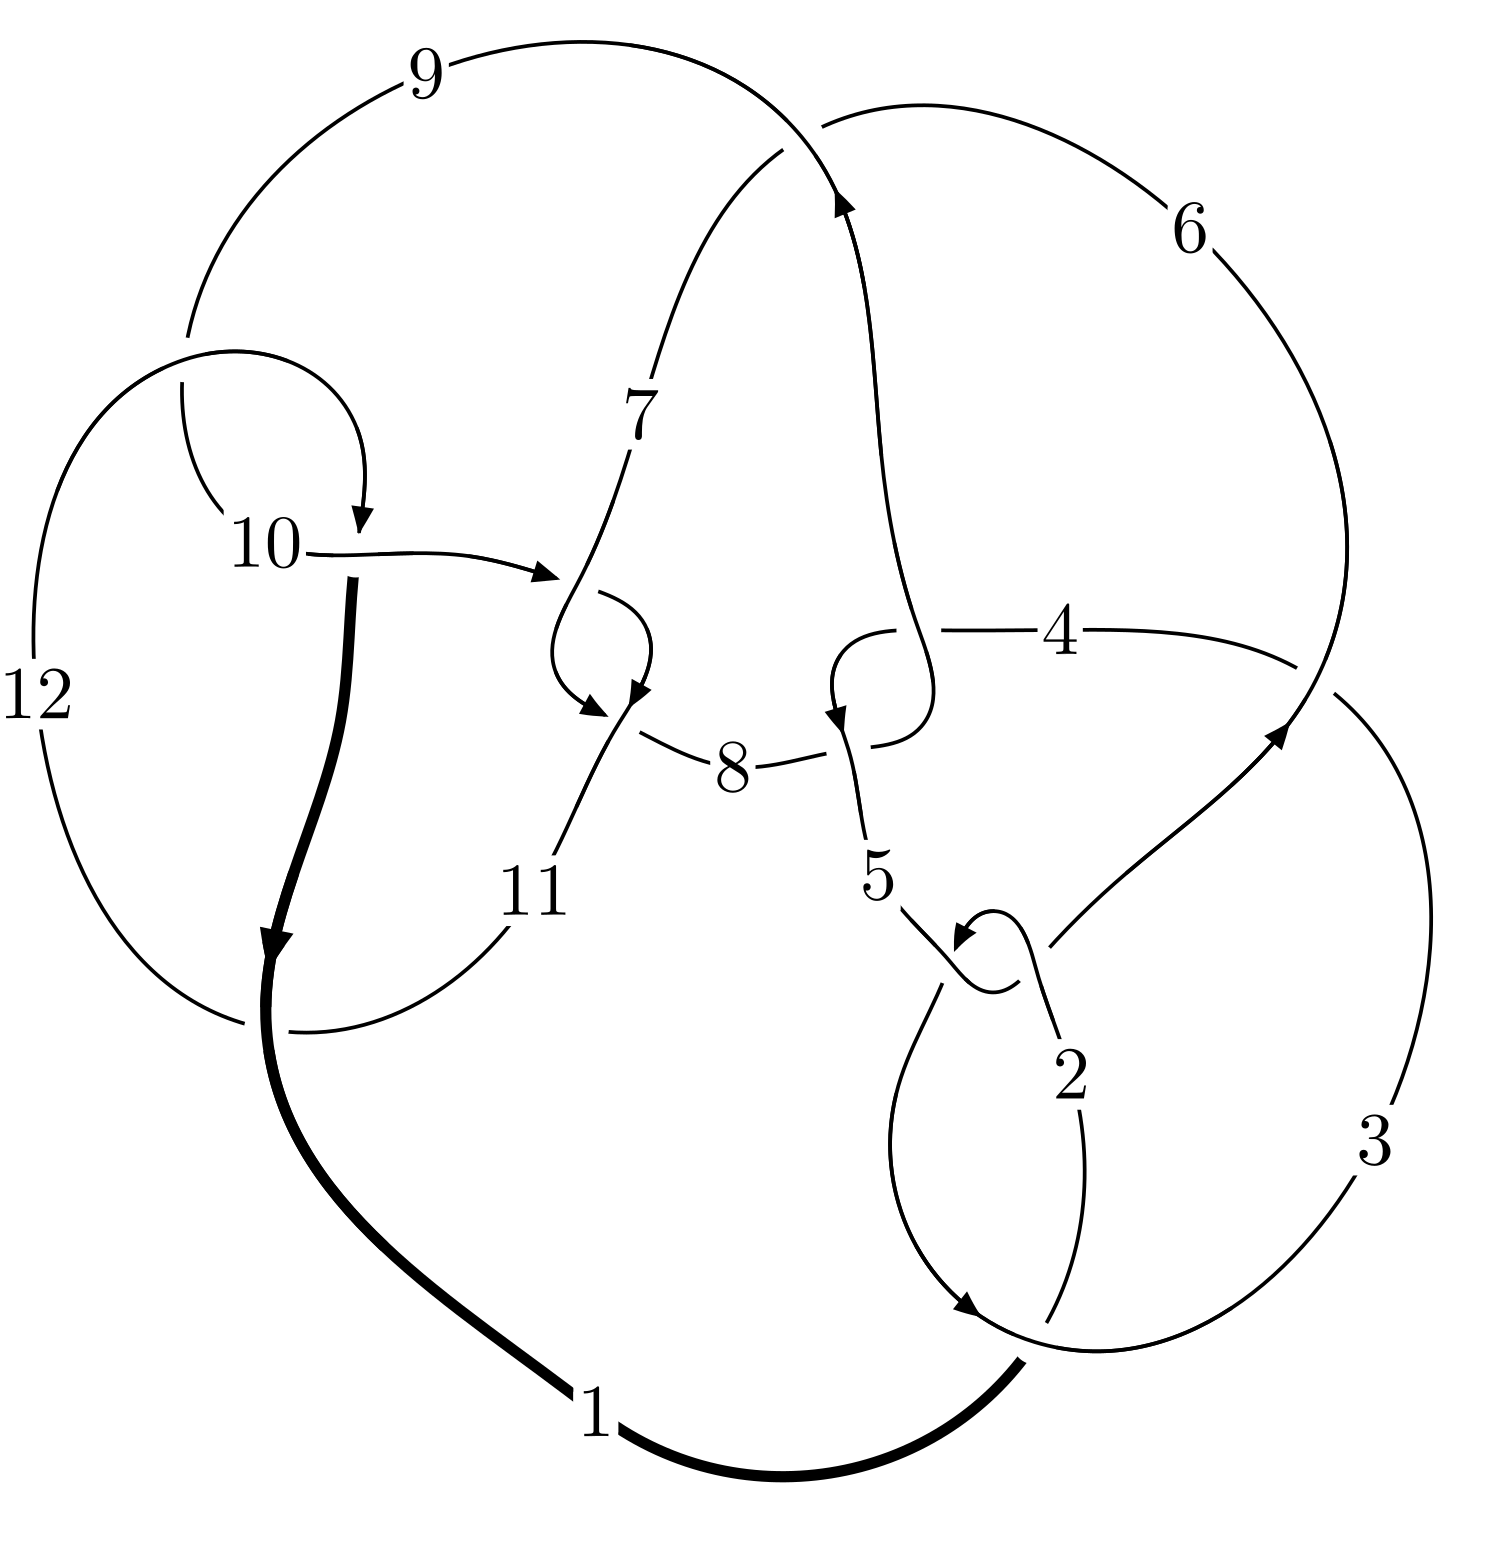
\includegraphics[width=112pt]{../../../GIT/diagram.site/Diagrams/png/2091_12n_0002.png}\\
\ \ \ A knot diagram\footnotemark}&
\allowdisplaybreaks
\textbf{Linearized knot diagam} \\
\cline{2-2}
 &
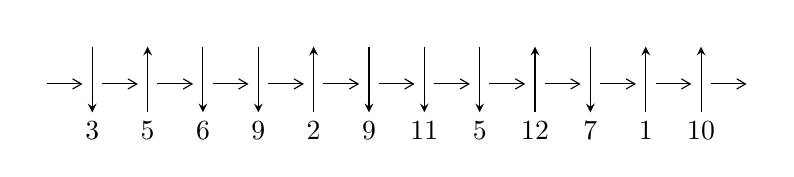
\begin{tikzpicture}[x=20pt, y=17pt]
	% nodes
	\node (C0) at (0, 0) {};
	\node (C1) at (1, 0) {};
	\node (C1U) at (1, +1) {};
	\node (C1D) at (1, -1) {3};

	\node (C2) at (2, 0) {};
	\node (C2U) at (2, +1) {};
	\node (C2D) at (2, -1) {5};

	\node (C3) at (3, 0) {};
	\node (C3U) at (3, +1) {};
	\node (C3D) at (3, -1) {6};

	\node (C4) at (4, 0) {};
	\node (C4U) at (4, +1) {};
	\node (C4D) at (4, -1) {9};

	\node (C5) at (5, 0) {};
	\node (C5U) at (5, +1) {};
	\node (C5D) at (5, -1) {2};

	\node (C6) at (6, 0) {};
	\node (C6U) at (6, +1) {};
	\node (C6D) at (6, -1) {9};

	\node (C7) at (7, 0) {};
	\node (C7U) at (7, +1) {};
	\node (C7D) at (7, -1) {11};

	\node (C8) at (8, 0) {};
	\node (C8U) at (8, +1) {};
	\node (C8D) at (8, -1) {5};

	\node (C9) at (9, 0) {};
	\node (C9U) at (9, +1) {};
	\node (C9D) at (9, -1) {12};

	\node (C10) at (10, 0) {};
	\node (C10U) at (10, +1) {};
	\node (C10D) at (10, -1) {7};

	\node (C11) at (11, 0) {};
	\node (C11U) at (11, +1) {};
	\node (C11D) at (11, -1) {1};

	\node (C12) at (12, 0) {};
	\node (C12U) at (12, +1) {};
	\node (C12D) at (12, -1) {10};
	\node (C13) at (13, 0) {};

	% arrows
	\draw[->,>={angle 60}]
	(C0) edge (C1) (C1) edge (C2) (C2) edge (C3) (C3) edge (C4) (C4) edge (C5) (C5) edge (C6) (C6) edge (C7) (C7) edge (C8) (C8) edge (C9) (C9) edge (C10) (C10) edge (C11) (C11) edge (C12) (C12) edge (C13) ;	\draw[->,>=stealth]
	(C1U) edge (C1D) (C2D) edge (C2U) (C3U) edge (C3D) (C4U) edge (C4D) (C5D) edge (C5U) (C6U) edge (C6D) (C7U) edge (C7D) (C8U) edge (C8D) (C9D) edge (C9U) (C10U) edge (C10D) (C11D) edge (C11U) (C12D) edge (C12U) ;
	\end{tikzpicture} \\
\hhline{~~} \\& 
\textbf{Solving Sequence} \\ \cline{2-2} 
 &
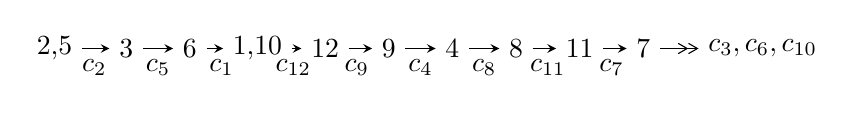
\begin{tikzpicture}[x=23pt, y=7pt]
	% node
	\node (A0) at (-1/8, 0) {2,5};
	\node (A1) at (1, 0) {3};
	\node (A2) at (2, 0) {6};
	\node (A3) at (49/16, 0) {1,10};
	\node (A4) at (33/8, 0) {12};
	\node (A5) at (41/8, 0) {9};
	\node (A6) at (49/8, 0) {4};
	\node (A7) at (57/8, 0) {8};
	\node (A8) at (65/8, 0) {11};
	\node (A9) at (73/8, 0) {7};
	\node (C1) at (1/2, -1) {$c_{2}$};
	\node (C2) at (3/2, -1) {$c_{5}$};
	\node (C3) at (5/2, -1) {$c_{1}$};
	\node (C4) at (29/8, -1) {$c_{12}$};
	\node (C5) at (37/8, -1) {$c_{9}$};
	\node (C6) at (45/8, -1) {$c_{4}$};
	\node (C7) at (53/8, -1) {$c_{8}$};
	\node (C8) at (61/8, -1) {$c_{11}$};
	\node (C9) at (69/8, -1) {$c_{7}$};
	\node (A10) at (11, 0) {$c_{3},c_{6},c_{10}$};

	% edge
	\draw[->,>=stealth]	
	(A0) edge (A1) (A1) edge (A2) (A2) edge (A3) (A3) edge (A4) (A4) edge (A5) (A5) edge (A6) (A6) edge (A7) (A7) edge (A8) (A8) edge (A9) ;
	\draw[->>,>={angle 60}]	
	(A9) edge (A10);
\end{tikzpicture} \\ 

\end{tabular} \\

\footnotetext{
The image of knot diagram is generated by the software ``\textbf{Draw programme}" developed by Andrew Bartholomew(\url{http://www.layer8.co.uk/maths/draw/index.htm\#Running-draw}), where we modified some parts for our purpose(\url{https://github.com/CATsTAILs/LinksPainter}).
}\phantom \\ \newline 
\centering \textbf{Ideals for irreducible components\footnotemark of $X_{\text{par}}$} 
 
\begin{align*}
I^u_{1}&=\langle 
1.50952\times10^{19} u^{57}-1.17965\times10^{20} u^{56}+\cdots+8.90580\times10^{18} b-7.29842\times10^{18},\\
\phantom{I^u_{1}}&\phantom{= \langle  }-1.00393\times10^{18} u^{57}+3.12591\times10^{18} u^{56}+\cdots+4.45290\times10^{18} a+3.47008\times10^{18},\;u^{58}-8 u^{57}+\cdots-2 u+1\rangle \\
I^u_{2}&=\langle 
- a^5+a^4 u+5 a^3 u+5 a^3+a^2-5 a u+3 b-3 a+u+1,\;a^6-4 a^4 u-4 a^4+a^3+4 a^2 u+1,\;u^2+u+1\rangle \\
I^u_{3}&=\langle 
- u^3+u^2+b-1,\;u^4- u^3+2 u^2+a,\;u^5- u^4+2 u^3- u^2+u-1\rangle \\
\\
\end{align*}
\raggedright * 3 irreducible components of $\dim_{\mathbb{C}}=0$, with total 75 representations.\\
\footnotetext{All coefficients of polynomials are rational numbers. But the coefficients are sometimes approximated in decimal forms when there is not enough margin.}
\newpage
\renewcommand{\arraystretch}{1}
\centering \section*{I. $I^u_{1}= \langle 1.51\times10^{19} u^{57}-1.18\times10^{20} u^{56}+\cdots+8.91\times10^{18} b-7.30\times10^{18},\;-1.00\times10^{18} u^{57}+3.13\times10^{18} u^{56}+\cdots+4.45\times10^{18} a+3.47\times10^{18},\;u^{58}-8 u^{57}+\cdots-2 u+1 \rangle$}
\flushleft \textbf{(i) Arc colorings}\\
\begin{tabular}{m{7pt} m{180pt} m{7pt} m{180pt} }
\flushright $a_{2}=$&$\begin{pmatrix}1\\0\end{pmatrix}$ \\
\flushright $a_{5}=$&$\begin{pmatrix}0\\u\end{pmatrix}$ \\
\flushright $a_{3}=$&$\begin{pmatrix}1\\- u^2\end{pmatrix}$ \\
\flushright $a_{6}=$&$\begin{pmatrix}u\\u\end{pmatrix}$ \\
\flushright $a_{1}=$&$\begin{pmatrix}u^2+1\\- u^4\end{pmatrix}$ \\
\flushright $a_{10}=$&$\begin{pmatrix}0.225455 u^{57}-0.701994 u^{56}+\cdots-6.72656 u-0.779286\\-1.69498 u^{57}+13.2459 u^{56}+\cdots-1.76418 u+0.819513\end{pmatrix}$ \\
\flushright $a_{12}=$&$\begin{pmatrix}-0.0574055 u^{57}-0.455661 u^{56}+\cdots+3.20301 u+1.10290\\0.153541 u^{57}-1.95463 u^{56}+\cdots+0.280763 u-0.208388\end{pmatrix}$ \\
\flushright $a_{9}=$&$\begin{pmatrix}-0.439374 u^{57}+3.08799 u^{56}+\cdots-7.87466 u-0.429764\\-1.22559 u^{57}+7.69945 u^{56}+\cdots+0.535607 u-0.892059\end{pmatrix}$ \\
\flushright $a_{4}=$&$\begin{pmatrix}u^4+u^2+1\\u^4\end{pmatrix}$ \\
\flushright $a_{8}=$&$\begin{pmatrix}-0.439374 u^{57}+3.08799 u^{56}+\cdots-7.87466 u-0.429764\\-2.54116 u^{57}+16.5796 u^{56}+\cdots+0.950230 u-1.31906\end{pmatrix}$ \\
\flushright $a_{11}=$&$\begin{pmatrix}-0.144303 u^{57}+0.234853 u^{56}+\cdots+4.42130 u+0.826807\\0.637447 u^{57}-5.42639 u^{56}+\cdots+1.41189 u-0.810401\end{pmatrix}$ \\
\flushright $a_{7}=$&$\begin{pmatrix}- u^2-1\\-0.0312500 u^{57}+0.218750 u^{56}+\cdots+1.03125 u^{2}+1.96875 u\end{pmatrix}$\\&\end{tabular}
\flushleft \textbf{(ii) Obstruction class $= -1$}\\~\\
\flushleft \textbf{(iii) Cusp Shapes $= \frac{11962378823504572851}{4452900487453949456} u^{57}-\frac{51305067713791607137}{2226450243726974728} u^{56}+\cdots+\frac{42176209722625714401}{4452900487453949456} u-\frac{11662141419335258151}{2226450243726974728}$}\\~\\
\newpage\renewcommand{\arraystretch}{1}
\flushleft \textbf{(iv) u-Polynomials at the component}\newline \\
\begin{tabular}{m{50pt}|m{274pt}}
Crossings & \hspace{64pt}u-Polynomials at each crossing \\
\hline $$\begin{aligned}c_{1}\end{aligned}$$&$\begin{aligned}
&u^{58}+36 u^{57}+\cdots+38 u+1
\end{aligned}$\\
\hline $$\begin{aligned}c_{2},c_{5}\end{aligned}$$&$\begin{aligned}
&u^{58}+8 u^{57}+\cdots+2 u+1
\end{aligned}$\\
\hline $$\begin{aligned}c_{3}\end{aligned}$$&$\begin{aligned}
&u^{58}-8 u^{57}+\cdots-10 u+1
\end{aligned}$\\
\hline $$\begin{aligned}c_{4},c_{8}\end{aligned}$$&$\begin{aligned}
&u^{58}+2 u^{57}+\cdots+22528 u^2-4096
\end{aligned}$\\
\hline $$\begin{aligned}c_{6}\end{aligned}$$&$\begin{aligned}
&u^{58}-4 u^{57}+\cdots+2 u-1
\end{aligned}$\\
\hline $$\begin{aligned}c_{7},c_{10}\end{aligned}$$&$\begin{aligned}
&u^{58}+3 u^{57}+\cdots+96 u+32
\end{aligned}$\\
\hline $$\begin{aligned}c_{9},c_{12}\end{aligned}$$&$\begin{aligned}
&u^{58}+8 u^{57}+\cdots-8 u-1
\end{aligned}$\\
\hline $$\begin{aligned}c_{11}\end{aligned}$$&$\begin{aligned}
&u^{58}-24 u^{57}+\cdots+160 u+1
\end{aligned}$\\
\hline
\end{tabular}\\~\\
\newpage\renewcommand{\arraystretch}{1}
\flushleft \textbf{(v) Riley Polynomials at the component}\newline \\
\begin{tabular}{m{50pt}|m{274pt}}
Crossings & \hspace{64pt}Riley Polynomials at each crossing \\
\hline $$\begin{aligned}c_{1}\end{aligned}$$&$\begin{aligned}
&y^{58}-20 y^{57}+\cdots+1622 y+1
\end{aligned}$\\
\hline $$\begin{aligned}c_{2},c_{5}\end{aligned}$$&$\begin{aligned}
&y^{58}+36 y^{57}+\cdots+38 y+1
\end{aligned}$\\
\hline $$\begin{aligned}c_{3}\end{aligned}$$&$\begin{aligned}
&y^{58}-76 y^{57}+\cdots+38 y+1
\end{aligned}$\\
\hline $$\begin{aligned}c_{4},c_{8}\end{aligned}$$&$\begin{aligned}
&y^{58}-70 y^{57}+\cdots-184549376 y+16777216
\end{aligned}$\\
\hline $$\begin{aligned}c_{6}\end{aligned}$$&$\begin{aligned}
&y^{58}-76 y^{57}+\cdots+34 y+1
\end{aligned}$\\
\hline $$\begin{aligned}c_{7},c_{10}\end{aligned}$$&$\begin{aligned}
&y^{58}-39 y^{57}+\cdots-11776 y+1024
\end{aligned}$\\
\hline $$\begin{aligned}c_{9},c_{12}\end{aligned}$$&$\begin{aligned}
&y^{58}-24 y^{57}+\cdots+160 y+1
\end{aligned}$\\
\hline $$\begin{aligned}c_{11}\end{aligned}$$&$\begin{aligned}
&y^{58}+28 y^{57}+\cdots-15092 y+1
\end{aligned}$\\
\hline
\end{tabular}\\~\\
\newpage\flushleft \textbf{(vi) Complex Volumes and Cusp Shapes}
$$\begin{array}{c|c|c}  
\text{Solutions to }I^u_{1}& \I (\text{vol} + \sqrt{-1}CS) & \text{Cusp shape}\\
 \hline 
\begin{aligned}
u &= \phantom{-}0.275952 + 0.968192 I \\
a &= -0.000155 + 0.297955 I \\
b &= \phantom{-}1.10303 - 1.31729 I\end{aligned}
 & -0.96404 + 7.38208 I & \phantom{-0.000000 } 0 \\ \hline\begin{aligned}
u &= \phantom{-}0.275952 - 0.968192 I \\
a &= -0.000155 - 0.297955 I \\
b &= \phantom{-}1.10303 + 1.31729 I\end{aligned}
 & -0.96404 - 7.38208 I & \phantom{-0.000000 } 0 \\ \hline\begin{aligned}
u &= \phantom{-}0.978634 + 0.050547 I \\
a &= -0.55182 + 2.57301 I \\
b &= \phantom{-}0.022208 - 0.782754 I\end{aligned}
 & -4.75178 - 2.65507 I & \phantom{-0.000000 } 0 \\ \hline\begin{aligned}
u &= \phantom{-}0.978634 - 0.050547 I \\
a &= -0.55182 - 2.57301 I \\
b &= \phantom{-}0.022208 + 0.782754 I\end{aligned}
 & -4.75178 + 2.65507 I & \phantom{-0.000000 } 0 \\ \hline\begin{aligned}
u &= \phantom{-}1.023510 + 0.155528 I \\
a &= -0.27153 - 2.55040 I \\
b &= \phantom{-}0.021646 + 0.911291 I\end{aligned}
 & -8.49450 - 9.39894 I & \phantom{-0.000000 } 0 \\ \hline\begin{aligned}
u &= \phantom{-}1.023510 - 0.155528 I \\
a &= -0.27153 + 2.55040 I \\
b &= \phantom{-}0.021646 - 0.911291 I\end{aligned}
 & -8.49450 + 9.39894 I & \phantom{-0.000000 } 0 \\ \hline\begin{aligned}
u &= \phantom{-}1.039610 + 0.094873 I \\
a &= \phantom{-}0.51869 + 1.62894 I \\
b &= \phantom{-}0.260631 - 0.513525 I\end{aligned}
 & -10.45060 - 3.04051 I & \phantom{-0.000000 } 0 \\ \hline\begin{aligned}
u &= \phantom{-}1.039610 - 0.094873 I \\
a &= \phantom{-}0.51869 - 1.62894 I \\
b &= \phantom{-}0.260631 + 0.513525 I\end{aligned}
 & -10.45060 + 3.04051 I & \phantom{-0.000000 } 0 \\ \hline\begin{aligned}
u &= \phantom{-}0.955917\phantom{ +0.000000I} \\
a &= \phantom{-}1.03957\phantom{ +0.000000I} \\
b &= -1.17742\phantom{ +0.000000I}\end{aligned}
 & -3.08584\phantom{ +0.000000I} & \phantom{-0.000000 } 0 \\ \hline\begin{aligned}
u &= -0.171249 + 1.030670 I \\
a &= -0.063866 + 0.965609 I \\
b &= \phantom{-}1.090800 + 0.593842 I\end{aligned}
 & -0.92134 - 2.15292 I & \phantom{-0.000000 } 0\\
 \hline 
 \end{array}$$\newpage$$\begin{array}{c|c|c}  
\text{Solutions to }I^u_{1}& \I (\text{vol} + \sqrt{-1}CS) & \text{Cusp shape}\\
 \hline 
\begin{aligned}
u &= -0.171249 - 1.030670 I \\
a &= -0.063866 - 0.965609 I \\
b &= \phantom{-}1.090800 - 0.593842 I\end{aligned}
 & -0.92134 + 2.15292 I & \phantom{-0.000000 } 0 \\ \hline\begin{aligned}
u &= \phantom{-}0.093713 + 0.946838 I \\
a &= -0.553562 - 0.684632 I \\
b &= -1.49296 + 1.41946 I\end{aligned}
 & \phantom{-}0.65102 + 1.70576 I & \phantom{-0.000000 } 0 \\ \hline\begin{aligned}
u &= \phantom{-}0.093713 - 0.946838 I \\
a &= -0.553562 + 0.684632 I \\
b &= -1.49296 - 1.41946 I\end{aligned}
 & \phantom{-}0.65102 - 1.70576 I & \phantom{-0.000000 } 0 \\ \hline\begin{aligned}
u &= -0.385585 + 0.867994 I \\
a &= -0.485247 + 0.372815 I \\
b &= -0.175174 + 0.510497 I\end{aligned}
 & -0.35129 - 1.66089 I & \phantom{-0.000000 } 0 \\ \hline\begin{aligned}
u &= -0.385585 - 0.867994 I \\
a &= -0.485247 - 0.372815 I \\
b &= -0.175174 - 0.510497 I\end{aligned}
 & -0.35129 + 1.66089 I & \phantom{-0.000000 } 0 \\ \hline\begin{aligned}
u &= -0.505582 + 0.803238 I \\
a &= -2.09011 - 2.61641 I \\
b &= -2.09154 - 2.96921 I\end{aligned}
 & \phantom{-}1.74781 - 1.62369 I & \phantom{-0.000000 -}0. + 24.7327 I \\ \hline\begin{aligned}
u &= -0.505582 - 0.803238 I \\
a &= -2.09011 + 2.61641 I \\
b &= -2.09154 + 2.96921 I\end{aligned}
 & \phantom{-}1.74781 + 1.62369 I & \phantom{-0.000000 } 0. - 24.7327 I \\ \hline\begin{aligned}
u &= -0.561420 + 0.898597 I \\
a &= \phantom{-}2.07464 + 1.60753 I \\
b &= \phantom{-}1.43908 + 1.62628 I\end{aligned}
 & \phantom{-}1.38531 - 2.69246 I & \phantom{-0.000000 } 0 \\ \hline\begin{aligned}
u &= -0.561420 - 0.898597 I \\
a &= \phantom{-}2.07464 - 1.60753 I \\
b &= \phantom{-}1.43908 - 1.62628 I\end{aligned}
 & \phantom{-}1.38531 + 2.69246 I & \phantom{-0.000000 } 0 \\ \hline\begin{aligned}
u &= -0.726204 + 0.589006 I \\
a &= \phantom{-}0.00616 + 1.68117 I \\
b &= -0.547028 + 1.145170 I\end{aligned}
 & -0.969194 + 0.999280 I & \phantom{-0.000000 } 0\\
 \hline 
 \end{array}$$\newpage$$\begin{array}{c|c|c}  
\text{Solutions to }I^u_{1}& \I (\text{vol} + \sqrt{-1}CS) & \text{Cusp shape}\\
 \hline 
\begin{aligned}
u &= -0.726204 - 0.589006 I \\
a &= \phantom{-}0.00616 - 1.68117 I \\
b &= -0.547028 - 1.145170 I\end{aligned}
 & -0.969194 - 0.999280 I & \phantom{-0.000000 } 0 \\ \hline\begin{aligned}
u &= \phantom{-}0.175532 + 1.051230 I \\
a &= \phantom{-}0.428231 - 0.504967 I \\
b &= \phantom{-}0.019179 - 0.580968 I\end{aligned}
 & -3.55927 + 2.47567 I & \phantom{-0.000000 } 0 \\ \hline\begin{aligned}
u &= \phantom{-}0.175532 - 1.051230 I \\
a &= \phantom{-}0.428231 + 0.504967 I \\
b &= \phantom{-}0.019179 + 0.580968 I\end{aligned}
 & -3.55927 - 2.47567 I & \phantom{-0.000000 } 0 \\ \hline\begin{aligned}
u &= -0.024346 + 0.878987 I \\
a &= -1.212630 + 0.073534 I \\
b &= -2.14746 + 0.60990 I\end{aligned}
 & \phantom{-}1.218520 - 0.673498 I & -4.18882 - 1.05925 I \\ \hline\begin{aligned}
u &= -0.024346 - 0.878987 I \\
a &= -1.212630 - 0.073534 I \\
b &= -2.14746 - 0.60990 I\end{aligned}
 & \phantom{-}1.218520 + 0.673498 I & -4.18882 + 1.05925 I \\ \hline\begin{aligned}
u &= -0.704127 + 0.981644 I \\
a &= -1.74849 + 0.22678 I \\
b &= -1.64792 - 0.60728 I\end{aligned}
 & -2.05852 - 6.41903 I & \phantom{-0.000000 } 0 \\ \hline\begin{aligned}
u &= -0.704127 - 0.981644 I \\
a &= -1.74849 - 0.22678 I \\
b &= -1.64792 + 0.60728 I\end{aligned}
 & -2.05852 + 6.41903 I & \phantom{-0.000000 } 0 \\ \hline\begin{aligned}
u &= -0.692017 + 0.375664 I \\
a &= \phantom{-}0.372198 - 0.642161 I \\
b &= \phantom{-}0.920888 - 0.097592 I\end{aligned}
 & -0.81151 - 3.99437 I & -2.30538 + 5.50801 I \\ \hline\begin{aligned}
u &= -0.692017 - 0.375664 I \\
a &= \phantom{-}0.372198 + 0.642161 I \\
b &= \phantom{-}0.920888 + 0.097592 I\end{aligned}
 & -0.81151 + 3.99437 I & -2.30538 - 5.50801 I \\ \hline\begin{aligned}
u &= -0.629338 + 1.046620 I \\
a &= \phantom{-}0.677631 - 0.327862 I \\
b &= \phantom{-}0.848161 + 0.573228 I\end{aligned}
 & -2.61151 - 1.02917 I & \phantom{-0.000000 } 0\\
 \hline 
 \end{array}$$\newpage$$\begin{array}{c|c|c}  
\text{Solutions to }I^u_{1}& \I (\text{vol} + \sqrt{-1}CS) & \text{Cusp shape}\\
 \hline 
\begin{aligned}
u &= -0.629338 - 1.046620 I \\
a &= \phantom{-}0.677631 + 0.327862 I \\
b &= \phantom{-}0.848161 - 0.573228 I\end{aligned}
 & -2.61151 + 1.02917 I & \phantom{-0.000000 } 0 \\ \hline\begin{aligned}
u &= -0.171554 + 1.234280 I \\
a &= \phantom{-}0.966951 - 0.171109 I \\
b &= \phantom{-}1.74065 - 1.48643 I\end{aligned}
 & -6.43951 - 0.95824 I & \phantom{-0.000000 } 0 \\ \hline\begin{aligned}
u &= -0.171554 - 1.234280 I \\
a &= \phantom{-}0.966951 + 0.171109 I \\
b &= \phantom{-}1.74065 + 1.48643 I\end{aligned}
 & -6.43951 + 0.95824 I & \phantom{-0.000000 } 0 \\ \hline\begin{aligned}
u &= \phantom{-}0.463795 + 1.173060 I \\
a &= \phantom{-}0.245701 - 0.546846 I \\
b &= \phantom{-}0.27203 - 1.99888 I\end{aligned}
 & -4.70507 + 4.20146 I & \phantom{-0.000000 } 0 \\ \hline\begin{aligned}
u &= \phantom{-}0.463795 - 1.173060 I \\
a &= \phantom{-}0.245701 + 0.546846 I \\
b &= \phantom{-}0.27203 + 1.99888 I\end{aligned}
 & -4.70507 - 4.20146 I & \phantom{-0.000000 } 0 \\ \hline\begin{aligned}
u &= -0.276279 + 1.243530 I \\
a &= -0.500340 - 0.211080 I \\
b &= -1.57432 + 1.01324 I\end{aligned}
 & -5.50368 - 7.01216 I & \phantom{-0.000000 } 0 \\ \hline\begin{aligned}
u &= -0.276279 - 1.243530 I \\
a &= -0.500340 + 0.211080 I \\
b &= -1.57432 - 1.01324 I\end{aligned}
 & -5.50368 + 7.01216 I & \phantom{-0.000000 } 0 \\ \hline\begin{aligned}
u &= \phantom{-}0.305286 + 0.606062 I \\
a &= \phantom{-}0.384294 + 0.040597 I \\
b &= \phantom{-}0.905016 - 1.068230 I\end{aligned}
 & \phantom{-}0.07617 - 4.63797 I & -3.02109 + 8.51541 I \\ \hline\begin{aligned}
u &= \phantom{-}0.305286 - 0.606062 I \\
a &= \phantom{-}0.384294 - 0.040597 I \\
b &= \phantom{-}0.905016 + 1.068230 I\end{aligned}
 & \phantom{-}0.07617 + 4.63797 I & -3.02109 - 8.51541 I \\ \hline\begin{aligned}
u &= \phantom{-}0.646890\phantom{ +0.000000I} \\
a &= -1.12299\phantom{ +0.000000I} \\
b &= \phantom{-}0.559207\phantom{ +0.000000I}\end{aligned}
 & -1.53774\phantom{ +0.000000I} & -8.16170\phantom{ +0.000000I}\\
 \hline 
 \end{array}$$\newpage$$\begin{array}{c|c|c}  
\text{Solutions to }I^u_{1}& \I (\text{vol} + \sqrt{-1}CS) & \text{Cusp shape}\\
 \hline 
\begin{aligned}
u &= \phantom{-}0.490058 + 1.298210 I \\
a &= -0.386776 + 0.469667 I \\
b &= -0.38414 + 2.46629 I\end{aligned}
 & -7.08177 + 5.14263 I & \phantom{-0.000000 } 0 \\ \hline\begin{aligned}
u &= \phantom{-}0.490058 - 1.298210 I \\
a &= -0.386776 - 0.469667 I \\
b &= -0.38414 - 2.46629 I\end{aligned}
 & -7.08177 - 5.14263 I & \phantom{-0.000000 } 0 \\ \hline\begin{aligned}
u &= \phantom{-}0.463084 + 1.320050 I \\
a &= -1.47034 - 0.97801 I \\
b &= -3.91851 - 1.65445 I\end{aligned}
 & -9.03269 + 2.43239 I & \phantom{-0.000000 } 0 \\ \hline\begin{aligned}
u &= \phantom{-}0.463084 - 1.320050 I \\
a &= -1.47034 + 0.97801 I \\
b &= -3.91851 + 1.65445 I\end{aligned}
 & -9.03269 - 2.43239 I & \phantom{-0.000000 } 0 \\ \hline\begin{aligned}
u &= \phantom{-}0.520231 + 1.298750 I \\
a &= \phantom{-}1.84530 + 0.28310 I \\
b &= \phantom{-}4.74633 + 0.27848 I\end{aligned}
 & -8.59701 + 8.01455 I & \phantom{-0.000000 } 0 \\ \hline\begin{aligned}
u &= \phantom{-}0.520231 - 1.298750 I \\
a &= \phantom{-}1.84530 - 0.28310 I \\
b &= \phantom{-}4.74633 - 0.27848 I\end{aligned}
 & -8.59701 - 8.01455 I & \phantom{-0.000000 } 0 \\ \hline\begin{aligned}
u &= \phantom{-}0.581889 + 1.286040 I \\
a &= -1.72412 - 0.78764 I \\
b &= -4.59705 - 1.31483 I\end{aligned}
 & -11.9798 + 15.1518 I & \phantom{-0.000000 } 0 \\ \hline\begin{aligned}
u &= \phantom{-}0.581889 - 1.286040 I \\
a &= -1.72412 + 0.78764 I \\
b &= -4.59705 + 1.31483 I\end{aligned}
 & -11.9798 - 15.1518 I & \phantom{-0.000000 } 0 \\ \hline\begin{aligned}
u &= \phantom{-}0.55851 + 1.31422 I \\
a &= \phantom{-}1.055310 + 0.777623 I \\
b &= \phantom{-}2.64117 + 1.02259 I\end{aligned}
 & -14.2321 + 8.7482 I & \phantom{-0.000000 } 0 \\ \hline\begin{aligned}
u &= \phantom{-}0.55851 - 1.31422 I \\
a &= \phantom{-}1.055310 - 0.777623 I \\
b &= \phantom{-}2.64117 - 1.02259 I\end{aligned}
 & -14.2321 - 8.7482 I & \phantom{-0.000000 } 0\\
 \hline 
 \end{array}$$\newpage$$\begin{array}{c|c|c}  
\text{Solutions to }I^u_{1}& \I (\text{vol} + \sqrt{-1}CS) & \text{Cusp shape}\\
 \hline 
\begin{aligned}
u &= \phantom{-}0.38902 + 1.37780 I \\
a &= \phantom{-}1.64061 + 0.55483 I \\
b &= \phantom{-}4.47101 + 0.66773 I\end{aligned}
 & -13.4742 - 4.4404 I & \phantom{-0.000000 } 0 \\ \hline\begin{aligned}
u &= \phantom{-}0.38902 - 1.37780 I \\
a &= \phantom{-}1.64061 - 0.55483 I \\
b &= \phantom{-}4.47101 - 0.66773 I\end{aligned}
 & -13.4742 + 4.4404 I & \phantom{-0.000000 } 0 \\ \hline\begin{aligned}
u &= \phantom{-}0.44158 + 1.37511 I \\
a &= -1.169000 - 0.047468 I \\
b &= -3.16209 - 0.19464 I\end{aligned}
 & -15.1541 + 2.2033 I & \phantom{-0.000000 } 0 \\ \hline\begin{aligned}
u &= \phantom{-}0.44158 - 1.37511 I \\
a &= -1.169000 + 0.047468 I \\
b &= -3.16209 + 0.19464 I\end{aligned}
 & -15.1541 - 2.2033 I & \phantom{-0.000000 } 0 \\ \hline\begin{aligned}
u &= \phantom{-}0.342722 + 0.311153 I \\
a &= -1.206810 + 0.383647 I \\
b &= \phantom{-}0.526147 + 0.412647 I\end{aligned}
 & -1.48988 - 0.34469 I & -6.13134 + 1.29951 I \\ \hline\begin{aligned}
u &= \phantom{-}0.342722 - 0.311153 I \\
a &= -1.206810 - 0.383647 I \\
b &= \phantom{-}0.526147 - 0.412647 I\end{aligned}
 & -1.48988 + 0.34469 I & -6.13134 - 1.29951 I \\ \hline\begin{aligned}
u &= -0.096823 + 0.143742 I \\
a &= -4.23922 - 1.64875 I \\
b &= -0.980677 + 0.184228 I\end{aligned}
 & \phantom{-}1.73915 - 0.71529 I & \phantom{-}3.95862 + 0.54158 I \\ \hline\begin{aligned}
u &= -0.096823 - 0.143742 I \\
a &= -4.23922 + 1.64875 I \\
b &= -0.980677 - 0.184228 I\end{aligned}
 & \phantom{-}1.73915 + 0.71529 I & \phantom{-}3.95862 - 0.54158 I\\
 \hline 
 \end{array}$$\newpage\newpage\renewcommand{\arraystretch}{1}
\centering \section*{II. $I^u_{2}= \langle a^4 u+5 a^3 u+\cdots-3 a+1,\;a^6-4 a^4 u-4 a^4+a^3+4 a^2 u+1,\;u^2+u+1 \rangle$}
\flushleft \textbf{(i) Arc colorings}\\
\begin{tabular}{m{7pt} m{180pt} m{7pt} m{180pt} }
\flushright $a_{2}=$&$\begin{pmatrix}1\\0\end{pmatrix}$ \\
\flushright $a_{5}=$&$\begin{pmatrix}0\\u\end{pmatrix}$ \\
\flushright $a_{3}=$&$\begin{pmatrix}1\\u+1\end{pmatrix}$ \\
\flushright $a_{6}=$&$\begin{pmatrix}u\\u\end{pmatrix}$ \\
\flushright $a_{1}=$&$\begin{pmatrix}- u\\- u\end{pmatrix}$ \\
\flushright $a_{10}=$&$\begin{pmatrix}a\\-\frac{1}{3} a^4 u-\frac{5}{3} a^3 u+\cdots+a-\frac{1}{3}\end{pmatrix}$ \\
\flushright $a_{12}=$&$\begin{pmatrix}-\frac{1}{3} a^5 u+\frac{2}{3} a^3 u+\cdots+\frac{1}{3} a^2-\frac{1}{3} a\\-\frac{1}{3} a^5 u+\frac{1}{3} a^4 u+\cdots-\frac{1}{3} a-\frac{2}{3}\end{pmatrix}$ \\
\flushright $a_{9}=$&$\begin{pmatrix}0\\\frac{1}{3} a^4 u-\frac{7}{3} a^3 u+\cdots+\frac{7}{3} a^2-\frac{5}{3}\end{pmatrix}$ \\
\flushright $a_{4}=$&$\begin{pmatrix}0\\u\end{pmatrix}$ \\
\flushright $a_{8}=$&$\begin{pmatrix}0\\\frac{1}{3} a^4 u-\frac{7}{3} a^3 u+\cdots+\frac{7}{3} a^2-\frac{5}{3}\end{pmatrix}$ \\
\flushright $a_{11}=$&$\begin{pmatrix}-\frac{2}{3} a^5 u+\frac{7}{3} a^3 u+\cdots+\frac{5}{3} a^2+\frac{4}{3} a\\-\frac{2}{3} a^5 u+\frac{1}{3} a^4 u+\cdots+\frac{4}{3} a-\frac{2}{3}\end{pmatrix}$ \\
\flushright $a_{7}=$&$\begin{pmatrix}u\\a^5+a^4 u-3 a^3 u-3 a^3+5 a^2+2 a u- u-2\end{pmatrix}$\\&\end{tabular}
\flushleft \textbf{(ii) Obstruction class $= 1$}\\~\\
\flushleft \textbf{(iii) Cusp Shapes $= 5 a^5 u+2 a^5+a^4 u-6 a^3 u+9 a^3+5 a^2 u+6 a^2-2 a u-6 a+2 u-4$}\\~\\
\newpage\renewcommand{\arraystretch}{1}
\flushleft \textbf{(iv) u-Polynomials at the component}\newline \\
\begin{tabular}{m{50pt}|m{274pt}}
Crossings & \hspace{64pt}u-Polynomials at each crossing \\
\hline $$\begin{aligned}c_{1},c_{3},c_{5}\end{aligned}$$&$\begin{aligned}
&(u^2- u+1)^6
\end{aligned}$\\
\hline $$\begin{aligned}c_{2}\end{aligned}$$&$\begin{aligned}
&(u^2+u+1)^6
\end{aligned}$\\
\hline $$\begin{aligned}c_{4},c_{8}\end{aligned}$$&$\begin{aligned}
&u^{12}
\end{aligned}$\\
\hline $$\begin{aligned}c_{6}\end{aligned}$$&$\begin{aligned}
&(u^6-3 u^5+5 u^4-4 u^3+2 u^2- u+1)^2
\end{aligned}$\\
\hline $$\begin{aligned}c_{7},c_{12}\end{aligned}$$&$\begin{aligned}
&(u^6+u^5- u^4-2 u^3+u+1)^2
\end{aligned}$\\
\hline $$\begin{aligned}c_{9},c_{10}\end{aligned}$$&$\begin{aligned}
&(u^6- u^5- u^4+2 u^3- u+1)^2
\end{aligned}$\\
\hline $$\begin{aligned}c_{11}\end{aligned}$$&$\begin{aligned}
&(u^6+3 u^5+5 u^4+4 u^3+2 u^2+u+1)^2
\end{aligned}$\\
\hline
\end{tabular}\\~\\
\newpage\renewcommand{\arraystretch}{1}
\flushleft \textbf{(v) Riley Polynomials at the component}\newline \\
\begin{tabular}{m{50pt}|m{274pt}}
Crossings & \hspace{64pt}Riley Polynomials at each crossing \\
\hline $$\begin{aligned}c_{1},c_{2},c_{3}\\c_{5}\end{aligned}$$&$\begin{aligned}
&(y^2+y+1)^6
\end{aligned}$\\
\hline $$\begin{aligned}c_{4},c_{8}\end{aligned}$$&$\begin{aligned}
&y^{12}
\end{aligned}$\\
\hline $$\begin{aligned}c_{6},c_{11}\end{aligned}$$&$\begin{aligned}
&(y^6+y^5+5 y^4+6 y^2+3 y+1)^2
\end{aligned}$\\
\hline $$\begin{aligned}c_{7},c_{9},c_{10}\\c_{12}\end{aligned}$$&$\begin{aligned}
&(y^6-3 y^5+5 y^4-4 y^3+2 y^2- y+1)^2
\end{aligned}$\\
\hline
\end{tabular}\\~\\
\newpage\flushleft \textbf{(vi) Complex Volumes and Cusp Shapes}
$$\begin{array}{c|c|c}  
\text{Solutions to }I^u_{2}& \I (\text{vol} + \sqrt{-1}CS) & \text{Cusp shape}\\
 \hline 
\begin{aligned}
u &= -0.500000 + 0.866025 I \\
a &= \phantom{-}0.984649 + 0.174545 I \\
b &= -0.036219 - 0.476146 I\end{aligned}
 & \phantom{-0.000000 } -7.72290 I & \phantom{-}0.57335 + 8.68103 I \\ \hline\begin{aligned}
u &= -0.500000 + 0.866025 I \\
a &= -0.643485 - 0.765459 I \\
b &= -0.69657 - 1.97490 I\end{aligned}
 & \phantom{-0.000000 -}3.66314 I & -3.68173 - 0.75872 I \\ \hline\begin{aligned}
u &= -0.500000 + 0.866025 I \\
a &= -0.532492 - 0.210196 I \\
b &= -0.171113 - 0.913331 I\end{aligned}
 & -1.89061 - 1.10558 I & -7.73749 + 2.70506 I \\ \hline\begin{aligned}
u &= -0.500000 + 0.866025 I \\
a &= \phantom{-}0.448281 + 0.356054 I \\
b &= -0.341341 + 0.317450 I\end{aligned}
 & -1.89061 - 2.95419 I & -4.53097 + 3.97184 I \\ \hline\begin{aligned}
u &= -0.500000 + 0.866025 I \\
a &= -1.62479 - 0.64137 I \\
b &= -0.867745 + 0.078785 I\end{aligned}
 & \phantom{-}1.89061 - 1.10558 I & \phantom{-}0.765607 + 0.616236 I \\ \hline\begin{aligned}
u &= -0.500000 + 0.866025 I \\
a &= \phantom{-}1.36783 + 1.08642 I \\
b &= \phantom{-}1.61298 + 2.10212 I\end{aligned}
 & \phantom{-}1.89061 - 2.95419 I & \phantom{-}4.61123 + 3.83711 I \\ \hline\begin{aligned}
u &= -0.500000 - 0.866025 I \\
a &= -0.643485 + 0.765459 I \\
b &= -0.69657 + 1.97490 I\end{aligned}
 & \phantom{-0.000000 -}7.72290 I & \phantom{-}0.57335 - 8.68103 I \\ \hline\begin{aligned}
u &= -0.500000 - 0.866025 I \\
a &= \phantom{-}0.984649 - 0.174545 I \\
b &= -0.036219 + 0.476146 I\end{aligned}
 & \phantom{-0.000000 } -3.66314 I & -3.68173 + 0.75872 I \\ \hline\begin{aligned}
u &= -0.500000 - 0.866025 I \\
a &= -0.532492 + 0.210196 I \\
b &= -0.171113 + 0.913331 I\end{aligned}
 & -1.89061 + 1.10558 I & -7.73749 - 2.70506 I \\ \hline\begin{aligned}
u &= -0.500000 - 0.866025 I \\
a &= \phantom{-}0.448281 - 0.356054 I \\
b &= -0.341341 - 0.317450 I\end{aligned}
 & -1.89061 + 2.95419 I & -4.53097 - 3.97184 I\\
 \hline 
 \end{array}$$\newpage$$\begin{array}{c|c|c}  
\text{Solutions to }I^u_{2}& \I (\text{vol} + \sqrt{-1}CS) & \text{Cusp shape}\\
 \hline 
\begin{aligned}
u &= -0.500000 - 0.866025 I \\
a &= -1.62479 + 0.64137 I \\
b &= -0.867745 - 0.078785 I\end{aligned}
 & \phantom{-}1.89061 + 1.10558 I & \phantom{-}0.765607 - 0.616236 I \\ \hline\begin{aligned}
u &= -0.500000 - 0.866025 I \\
a &= \phantom{-}1.36783 - 1.08642 I \\
b &= \phantom{-}1.61298 - 2.10212 I\end{aligned}
 & \phantom{-}1.89061 + 2.95419 I & \phantom{-}4.61123 - 3.83711 I\\
 \hline 
 \end{array}$$\newpage\newpage\renewcommand{\arraystretch}{1}
\centering \section*{III. $I^u_{3}= \langle - u^3+u^2+b-1,\;u^4- u^3+2 u^2+a,\;u^5- u^4+2 u^3- u^2+u-1 \rangle$}
\flushleft \textbf{(i) Arc colorings}\\
\begin{tabular}{m{7pt} m{180pt} m{7pt} m{180pt} }
\flushright $a_{2}=$&$\begin{pmatrix}1\\0\end{pmatrix}$ \\
\flushright $a_{5}=$&$\begin{pmatrix}0\\u\end{pmatrix}$ \\
\flushright $a_{3}=$&$\begin{pmatrix}1\\- u^2\end{pmatrix}$ \\
\flushright $a_{6}=$&$\begin{pmatrix}u\\u\end{pmatrix}$ \\
\flushright $a_{1}=$&$\begin{pmatrix}u^2+1\\- u^4\end{pmatrix}$ \\
\flushright $a_{10}=$&$\begin{pmatrix}- u^4+u^3-2 u^2\\u^3- u^2+1\end{pmatrix}$ \\
\flushright $a_{12}=$&$\begin{pmatrix}- u^4+u^3- u^2+1\\- u^4+u^3- u^2+1\end{pmatrix}$ \\
\flushright $a_{9}=$&$\begin{pmatrix}- u^2-1\\u^4\end{pmatrix}$ \\
\flushright $a_{4}=$&$\begin{pmatrix}u^4+u^2+1\\u^4\end{pmatrix}$ \\
\flushright $a_{8}=$&$\begin{pmatrix}- u^2-1\\2 u^4+u^2\end{pmatrix}$ \\
\flushright $a_{11}=$&$\begin{pmatrix}- u^4+u^3-2 u^2\\u^3- u^2+1\end{pmatrix}$ \\
\flushright $a_{7}=$&$\begin{pmatrix}- u^2-1\\2 u^4+u^2\end{pmatrix}$\\&\end{tabular}
\flushleft \textbf{(ii) Obstruction class $= 1$}\\~\\
\flushleft \textbf{(iii) Cusp Shapes $= 3 u^4+3 u^3-4 u^2+8 u-3$}\\~\\
\newpage\renewcommand{\arraystretch}{1}
\flushleft \textbf{(iv) u-Polynomials at the component}\newline \\
\begin{tabular}{m{50pt}|m{274pt}}
Crossings & \hspace{64pt}u-Polynomials at each crossing \\
\hline $$\begin{aligned}c_{1}\end{aligned}$$&$\begin{aligned}
&u^5-3 u^4+4 u^3- u^2- u+1
\end{aligned}$\\
\hline $$\begin{aligned}c_{2}\end{aligned}$$&$\begin{aligned}
&u^5- u^4+2 u^3- u^2+u-1
\end{aligned}$\\
\hline $$\begin{aligned}c_{3},c_{4}\end{aligned}$$&$\begin{aligned}
&u^5+u^4-2 u^3- u^2+u-1
\end{aligned}$\\
\hline $$\begin{aligned}c_{5}\end{aligned}$$&$\begin{aligned}
&u^5+u^4+2 u^3+u^2+u+1
\end{aligned}$\\
\hline $$\begin{aligned}c_{6}\end{aligned}$$&$\begin{aligned}
&u^5-5 u^4+8 u^3-3 u^2- u-1
\end{aligned}$\\
\hline $$\begin{aligned}c_{7},c_{10}\end{aligned}$$&$\begin{aligned}
&u^5
\end{aligned}$\\
\hline $$\begin{aligned}c_{8}\end{aligned}$$&$\begin{aligned}
&u^5- u^4-2 u^3+u^2+u+1
\end{aligned}$\\
\hline $$\begin{aligned}c_{9},c_{11}\end{aligned}$$&$\begin{aligned}
&(u+1)^5
\end{aligned}$\\
\hline $$\begin{aligned}c_{12}\end{aligned}$$&$\begin{aligned}
&(u-1)^5
\end{aligned}$\\
\hline
\end{tabular}\\~\\
\newpage\renewcommand{\arraystretch}{1}
\flushleft \textbf{(v) Riley Polynomials at the component}\newline \\
\begin{tabular}{m{50pt}|m{274pt}}
Crossings & \hspace{64pt}Riley Polynomials at each crossing \\
\hline $$\begin{aligned}c_{1}\end{aligned}$$&$\begin{aligned}
&y^5- y^4+8 y^3-3 y^2+3 y-1
\end{aligned}$\\
\hline $$\begin{aligned}c_{2},c_{5}\end{aligned}$$&$\begin{aligned}
&y^5+3 y^4+4 y^3+y^2- y-1
\end{aligned}$\\
\hline $$\begin{aligned}c_{3},c_{4},c_{8}\end{aligned}$$&$\begin{aligned}
&y^5-5 y^4+8 y^3-3 y^2- y-1
\end{aligned}$\\
\hline $$\begin{aligned}c_{6}\end{aligned}$$&$\begin{aligned}
&y^5-9 y^4+32 y^3-35 y^2-5 y-1
\end{aligned}$\\
\hline $$\begin{aligned}c_{7},c_{10}\end{aligned}$$&$\begin{aligned}
&y^5
\end{aligned}$\\
\hline $$\begin{aligned}c_{9},c_{11},c_{12}\end{aligned}$$&$\begin{aligned}
&(y-1)^5
\end{aligned}$\\
\hline
\end{tabular}\\~\\
\newpage\flushleft \textbf{(vi) Complex Volumes and Cusp Shapes}
$$\begin{array}{c|c|c}  
\text{Solutions to }I^u_{3}& \I (\text{vol} + \sqrt{-1}CS) & \text{Cusp shape}\\
 \hline 
\begin{aligned}
u &= -0.339110 + 0.822375 I \\
a &= \phantom{-}1.76766 + 0.21690 I \\
b &= \phantom{-}2.21033 + 0.28529 I\end{aligned}
 & \phantom{-}1.31583 - 1.53058 I & -1.50865 + 9.87103 I \\ \hline\begin{aligned}
u &= -0.339110 - 0.822375 I \\
a &= \phantom{-}1.76766 - 0.21690 I \\
b &= \phantom{-}2.21033 - 0.28529 I\end{aligned}
 & \phantom{-}1.31583 + 1.53058 I & -1.50865 - 9.87103 I \\ \hline\begin{aligned}
u &= \phantom{-}0.766826\phantom{ +0.000000I} \\
a &= -1.07090\phantom{ +0.000000I} \\
b &= \phantom{-}0.862888\phantom{ +0.000000I}\end{aligned}
 & -0.756147\phantom{ +0.000000I} & \phantom{-}3.17260\phantom{ +0.000000I} \\ \hline\begin{aligned}
u &= \phantom{-}0.455697 + 1.200150 I \\
a &= \phantom{-}0.267792 - 0.471915 I \\
b &= \phantom{-}0.35822 - 2.07480 I\end{aligned}
 & -4.22763 + 4.40083 I & \phantom{-}0.92237 - 5.80708 I \\ \hline\begin{aligned}
u &= \phantom{-}0.455697 - 1.200150 I \\
a &= \phantom{-}0.267792 + 0.471915 I \\
b &= \phantom{-}0.35822 + 2.07480 I\end{aligned}
 & -4.22763 - 4.40083 I & \phantom{-}0.92237 + 5.80708 I\\
 \hline 
 \end{array}$$\newpage
\newpage\renewcommand{\arraystretch}{1}
\centering \section*{ IV. u-Polynomials}
\begin{tabular}{m{50pt}|m{274pt}}
Crossings & \hspace{64pt}u-Polynomials at each crossing \\
\hline $$\begin{aligned}c_{1}\end{aligned}$$&$\begin{aligned}
&((u^2- u+1)^6)(u^5-3 u^4+\cdots- u+1)(u^{58}+36 u^{57}+\cdots+38 u+1)
\end{aligned}$\\
\hline $$\begin{aligned}c_{2}\end{aligned}$$&$\begin{aligned}
&((u^2+u+1)^6)(u^5- u^4+\cdots+u-1)(u^{58}+8 u^{57}+\cdots+2 u+1)
\end{aligned}$\\
\hline $$\begin{aligned}c_{3}\end{aligned}$$&$\begin{aligned}
&((u^2- u+1)^6)(u^5+u^4+\cdots+u-1)(u^{58}-8 u^{57}+\cdots-10 u+1)
\end{aligned}$\\
\hline $$\begin{aligned}c_{4}\end{aligned}$$&$\begin{aligned}
&u^{12}(u^5+u^4+\cdots+u-1)(u^{58}+2 u^{57}+\cdots+22528 u^{2}-4096)
\end{aligned}$\\
\hline $$\begin{aligned}c_{5}\end{aligned}$$&$\begin{aligned}
&((u^2- u+1)^6)(u^5+u^4+\cdots+u+1)(u^{58}+8 u^{57}+\cdots+2 u+1)
\end{aligned}$\\
\hline $$\begin{aligned}c_{6}\end{aligned}$$&$\begin{aligned}
&(u^5-5 u^4+8 u^3-3 u^2- u-1)(u^6-3 u^5+5 u^4-4 u^3+2 u^2- u+1)^2\\
&\cdot(u^{58}-4 u^{57}+\cdots+2 u-1)
\end{aligned}$\\
\hline $$\begin{aligned}c_{7}\end{aligned}$$&$\begin{aligned}
&u^5(u^6+u^5+\cdots+u+1)^{2}(u^{58}+3 u^{57}+\cdots+96 u+32)
\end{aligned}$\\
\hline $$\begin{aligned}c_{8}\end{aligned}$$&$\begin{aligned}
&u^{12}(u^5- u^4+\cdots+u+1)(u^{58}+2 u^{57}+\cdots+22528 u^{2}-4096)
\end{aligned}$\\
\hline $$\begin{aligned}c_{9}\end{aligned}$$&$\begin{aligned}
&((u+1)^5)(u^6- u^5+\cdots- u+1)^{2}(u^{58}+8 u^{57}+\cdots-8 u-1)
\end{aligned}$\\
\hline $$\begin{aligned}c_{10}\end{aligned}$$&$\begin{aligned}
&u^5(u^6- u^5+\cdots- u+1)^{2}(u^{58}+3 u^{57}+\cdots+96 u+32)
\end{aligned}$\\
\hline $$\begin{aligned}c_{11}\end{aligned}$$&$\begin{aligned}
&(u+1)^5(u^6+3 u^5+5 u^4+4 u^3+2 u^2+u+1)^2\\
&\cdot(u^{58}-24 u^{57}+\cdots+160 u+1)
\end{aligned}$\\
\hline $$\begin{aligned}c_{12}\end{aligned}$$&$\begin{aligned}
&((u-1)^5)(u^6+u^5+\cdots+u+1)^{2}(u^{58}+8 u^{57}+\cdots-8 u-1)
\end{aligned}$\\
\hline
\end{tabular}\newpage\renewcommand{\arraystretch}{1}
\centering \section*{ V. Riley Polynomials}
\begin{tabular}{m{50pt}|m{274pt}}
Crossings & \hspace{64pt}Riley Polynomials at each crossing \\
\hline $$\begin{aligned}c_{1}\end{aligned}$$&$\begin{aligned}
&(y^2+y+1)^6(y^5- y^4+8 y^3-3 y^2+3 y-1)\\
&\cdot(y^{58}-20 y^{57}+\cdots+1622 y+1)
\end{aligned}$\\
\hline $$\begin{aligned}c_{2},c_{5}\end{aligned}$$&$\begin{aligned}
&((y^2+y+1)^6)(y^5+3 y^4+\cdots- y-1)(y^{58}+36 y^{57}+\cdots+38 y+1)
\end{aligned}$\\
\hline $$\begin{aligned}c_{3}\end{aligned}$$&$\begin{aligned}
&(y^2+y+1)^6(y^5-5 y^4+8 y^3-3 y^2- y-1)\\
&\cdot(y^{58}-76 y^{57}+\cdots+38 y+1)
\end{aligned}$\\
\hline $$\begin{aligned}c_{4},c_{8}\end{aligned}$$&$\begin{aligned}
&y^{12}(y^5-5 y^4+8 y^3-3 y^2- y-1)\\
&\cdot(y^{58}-70 y^{57}+\cdots-184549376 y+16777216)
\end{aligned}$\\
\hline $$\begin{aligned}c_{6}\end{aligned}$$&$\begin{aligned}
&(y^5-9 y^4+32 y^3-35 y^2-5 y-1)(y^6+y^5+5 y^4+6 y^2+3 y+1)^2\\
&\cdot(y^{58}-76 y^{57}+\cdots+34 y+1)
\end{aligned}$\\
\hline $$\begin{aligned}c_{7},c_{10}\end{aligned}$$&$\begin{aligned}
&y^5(y^6-3 y^5+5 y^4-4 y^3+2 y^2- y+1)^2\\
&\cdot(y^{58}-39 y^{57}+\cdots-11776 y+1024)
\end{aligned}$\\
\hline $$\begin{aligned}c_{9},c_{12}\end{aligned}$$&$\begin{aligned}
&(y-1)^5(y^6-3 y^5+5 y^4-4 y^3+2 y^2- y+1)^2\\
&\cdot(y^{58}-24 y^{57}+\cdots+160 y+1)
\end{aligned}$\\
\hline $$\begin{aligned}c_{11}\end{aligned}$$&$\begin{aligned}
&(y-1)^5(y^6+y^5+5 y^4+6 y^2+3 y+1)^2\\
&\cdot(y^{58}+28 y^{57}+\cdots-15092 y+1)
\end{aligned}$\\
\hline
\end{tabular}
\vskip 2pc
\end{document}